\documentclass[10pt,twocolumn]{article}

\usepackage[margin=0.85in]{geometry}
\usepackage{times}
\usepackage{hyperref}
\usepackage{xcolor}
\usepackage{booktabs}
\usepackage{graphicx}
\usepackage{enumitem}
\hypersetup{colorlinks=true, linkcolor=blue!50!black, citecolor=blue!50!black,
            urlcolor=blue!50!black}

% Generated metric macros. Every quantitative value in this paper comes from
% here; the source is regenerated by `make reproduce`. See figures/metrics.tex.
% Auto-generated by experiments/metrics.py. Do not edit by hand.
% Every macro traces to a run_id in experiments/*/logs/.
\newcommand{\interopMean}{2.45}
\newcommand{\interopN}{1}
\newcommand{\interopRunID}{demo-20260830-233514-b269c1}
\newcommand{\fleetMean}{10.56}
\newcommand{\fleetRunID}{uc3-20260830-233527-1946}
\newcommand{\advDetections}{5/5}
\newcommand{\advNTests}{7}
\newcommand{\advControl}{passed}
\newcommand{\overheadSeconds}{1.37}
\newcommand{\overheadTasks}{5}
\newcommand{\overheadTokens}{1080}
\newcommand{\evLoopRate}{100}
\newcommand{\evBaselineRate}{0}
\newcommand{\triggerRate}{N/A}
\newcommand{\triggerN}{0}
\newcommand{\triggerReason}{not run}


\newcommand{\runid}[1]{\footnote{Regenerated from run \texttt{#1}; see
  \texttt{experiments/results/metrics.json}.}}

\title{\vspace{-2em}The Loop: A File-First Standard for Governed,
Portable Agent Self-Improvement}
\author{Minhal \\ \small (working name: \texttt{agentloop}; final naming pending)}
\date{2026}

\begin{document}
\maketitle

\begin{abstract}
Deployed agents learn during work, but that experience does not compound.
A lesson either dies with the context or persists ungoverned---an
unchecked memory write or prompt edit with no evidence, no gate, no audit
trail, and no path to any other agent. We present \emph{the Loop}, an open
standard that makes one self-modification \emph{proven, gated, recorded,
reversible, and portable}. The standard defines five objects (ChangeSet,
Evidence, Policy, Journal, Registry), a six-state lifecycle, four trust
levels, and six normative invariants, over a plain-file representation that
any agent able to read and write files can adopt. Enforcement is
deterministic code, never the model: a model must not be the gatekeeper of
its own change. We describe a reference executor, a conformance suite that
any implementation can run, two low-friction adoption doors (a drop-in
Claude Code skill and a Python SDK), and a Team-lite registry with
detached \texttt{ed25519} signatures. We evaluate the system with five
executed battle-test scenarios, an adversarial suite of real attacks, and
a reproducible experiments framework. Under the loop, \evLoopRate\% of
managed-file changes carry evidence versus \evBaselineRate\% in an
ungoverned baseline; all \advDetections{} modelled threats are stopped
while a legitimate control change passes; and one lesson crosses two
independent runtimes in \interopMean~s. Every number in this paper is
generated from logged runs by script.
\end{abstract}

\section{Problem}
\label{sec:problem}
Agent experience does not compound. Every deployed agent learns during
work. Then one of two bad things happens. Path one: the context ends and
the lesson dies. Path two: the lesson persists as a memory write, a prompt
edit, or a saved skill---with no evidence, no gate, no audit trail, and no
way to reach any other agent. Agents forget what they should keep, and keep
what nobody checked.

Two forces make this urgent. First, self-improving agent systems are no
longer hypothetical: evolutionary and reflective optimizers now rewrite
prompts and code automatically~\cite{alphaevolve,gepa,dspy}. Second, the
danger of ungoverned self-modification is documented. The Darwin G\"odel
Machine was observed to game its own evaluation, editing the very markers
meant to detect misbehaviour~\cite{dgm}. A system that grades its own
homework and then acts on the grade is not safe to run unattended.

This standard supplies the missing infrastructure for the fast improvement
loop: a unit of improvement, a proof, a brake, a record, and a
distribution channel. It does not make models smarter. It makes a change
proven, gated, recorded, reversible, and portable.

\paragraph{Contributions.} We contribute: (i) a file-first protocol for
governed self-improvement, defined by five objects, a lifecycle, four trust
levels, and six invariants, published under an open specification licence
with normative JSON Schemas; (ii) a reference executor and a conformance
suite that any independent implementation can run, including
required-failure cases and a deliberately broken executor that must fail;
(iii) two adoption doors that produce identical files---a drop-in harness
package with hook-level enforcement, and an SDK; (iv) an executed
evaluation: five battle-test scenarios, an adversarial suite of real
attacks with a control, and a reproducible experiments framework in which
every reported number regenerates from logged runs.

\paragraph{What this is not.} The standard does not make models smarter,
define agent-to-agent messaging~\cite{a2a}, define tool access~\cite{mcp},
or choose anyone's metrics. It makes the evidence portable and the change
governable.

\section{Design}
\label{sec:design}

\subsection{Design principles}
Four commitments shape everything else.
\textbf{Files first.} The Core representation is a directory of plain
files: no server, no daemon. Any agent that can read and write files can
participate. This is the lesson of \texttt{AGENTS.md}~\cite{agentsmd}:
adoption follows the format people already have.
\textbf{Instruction is not enforcement.} A skill is advisory text; a
model that is asked to respect a gate can decline. Only deterministic code
may enforce.
\textbf{Govern what already exists.} The change targets are the files that
already steer agents, so adoption requires zero migration.
\textbf{Reuse formats.} Provenance wraps in-toto and SLSA
concepts~\cite{intoto,slsa}; evidence points at Inspect~\cite{inspect} and
the EleutherAI harness~\cite{lmeval}; telemetry uses OpenTelemetry GenAI
conventions~\cite{otelgenai}; the journal follows transparency-log
design~\cite{rfc6962}. The standard invents a wrapper, not a world.

\subsection{Three change layers}
The loop governs the files that already steer agents:
\emph{context} (instructions and memory: \texttt{AGENTS.md},
\texttt{CLAUDE.md}, memory files)~\cite{agentsmd}; \emph{capability}
(executable skills and tool code); and \emph{architecture} (the agent
graph and its policies). Model weights are out of scope; a weight update
is recordable only as an opaque journal entry.

\subsection{The five objects}
A \textbf{ChangeSet} is the portable unit of improvement: a typed envelope
naming its layer, target files, a payload (a unified diff, a folder, or an
opaque reference), an origin, a rationale, and a list of evidence records.
\textbf{Evidence} records support a change; each names a kind, a grader
(\texttt{self} or \texttt{independent}), and a format that reuses existing
schemas---UK AISI Inspect logs~\cite{inspect}, the EleutherAI
harness~\cite{lmeval}, OpenTelemetry GenAI spans~\cite{otelgenai}, human
feedback, and a cheap \texttt{command-transcript} (run the failing command,
apply the change, run it again). \textbf{Policy} is the declared change
envelope: per layer, a trust level, a list of gates, and an allowlist of
target globs, plus a protected list and escalation/de-escalation rules.
The \textbf{Journal} is an append-only, hash-chained NDJSON log; each entry
carries the SHA-256 of the previous line, so any edit breaks
verification---the Core analogue of a transparency log~\cite{rfc6962}. The
\textbf{Registry} (Team profile) distributes accepted ChangeSets through a
plain git remote; a pulled ChangeSet never bypasses local gates.

\subsection{The file plane}
The normative Core representation is one directory:

\begin{verbatim}
.loop/
  policy.yaml        # the declared envelope
  journal/
    2026-08.ndjson   # append-only, hash-chained
  changesets/
    cs-20260830-a1b2/
      changeset.json # typed envelope
      payload.patch  # diff against targets
      evidence/
        ev-001.json  # evidence records
  state.json         # executor-managed
  registry.yaml      # Team profile only
\end{verbatim}

Three rules make this safe. \texttt{.loop/} is never a valid change target.
Targets must be under version control, or the executor snapshots them
before apply. Journal entries reference content hashes, and git commits
when present.

\subsection{Lifecycle and trust levels}
A ChangeSet moves \textsc{proposed} $\rightarrow$ \textsc{validated}
$\rightarrow$ \textsc{gated} $\rightarrow$ \textsc{applied}
$\rightarrow$ \textsc{observed} $\rightarrow$ \textsc{promoted}, with
\textsc{rejected} and \textsc{rolled\_back} branches:

\begin{verbatim}
PROPOSED -> VALIDATED -> GATED -> APPLIED
              |            |        |
              +- REJECTED -+        v
                                 OBSERVED
                                    |
                                    v
                                 PROMOTED
   ROLLED_BACK <- (APPLIED|OBSERVED|PROMOTED)
\end{verbatim}

\textsc{validated} checks schema, target allowlist, protected paths, and
the payload hash. \textsc{gated} evaluates policy: auto-approve, queue for
a human, or reject. \textsc{applied} snapshots the targets, applies the
payload, and journals before/after hashes. Rollback is reachable from
every post-apply state with one command.

Four trust levels govern each layer: L0 (suggest only), L1 (queue for a
human), L2 (automatic gates apply), L3 (full autonomy inside the
envelope). Defaults: context L2, capability L1, architecture L1. Rollback
and the journal are mandatory at every level, including L0---proposals are
journaled even when nothing applies.

\subsection{The ratchet turns both ways}
Autonomy is earned and lost by recorded behaviour, not by assertion.
Policy may declare escalation (raise a class after a track record of
applied changes with few rollbacks) and de-escalation (lower it after
repeated rollbacks in a window). De-escalation is mandatory where declared,
and both transitions are journaled. Crucially, the executor never rewrites
\texttt{policy.yaml}: the declared policy stays human-owned, and the
\emph{effective} level lives in executor state. This is how the system
honours two constraints that look contradictory---``only a human may change
policy'' and ``de-escalation is automatic''---without letting the agent
touch its own envelope.

\subsection{Invariants}
Six normative invariants hold the design together: (I1) the loop never
targets its own \texttt{.loop/} files; (I2) the journal is append-only and
hash-chained; (I3) L2/L3 application requires at least one
\emph{independent} evidence record; (I4) targets outside the allowlist
fail validation; (I5) every applied change is reversible with one command;
(I6, Team+) a distributor serves only signed ChangeSets. I3 is the direct
answer to eval-gaming~\cite{dgm}: the producer can never be the only
grader above L1.

\subsection{Enforcement is code, not instruction}
A skill can \emph{teach} the loop; only deterministic code may
\emph{enforce} it. The reference executor validates, gates, applies,
journals, and rolls back; the model cannot rewrite it mid-session, and
\texttt{.loop/} is protected. The universal backstop is one CI command,
\texttt{agentloop verify}, which checks that every diff to a managed target
has a matching valid journal entry and that the hash chain is intact---so
the guarantee is harness-independent.

\section{Implementation}
\label{sec:impl}
The reference executor is a Python~3.11 CLI (\texttt{agentloop}, alias
\texttt{loop}) and a library the SDK shares, so both adoption doors produce
identical files. Provenance and signing reuse existing supply-chain
practice in spirit~\cite{intoto,slsa,sigstore}; the v1 Team-lite profile
implements detached \texttt{ed25519} signatures over a canonical
ChangeSet digest, with verification on pull.

\paragraph{Two doors.} The \emph{consumer door} is a drop-in Claude Code
package: a skill that carries the cognition (when you learn a durable
lesson, propose---never edit managed files directly), a \texttt{PreToolUse}
hook that denies direct edits to managed targets and points at
\texttt{agentloop propose}, and a session-end reminder for queued changes.
Codex-class harnesses that lack hooks get an idempotent managed block in
\texttt{AGENTS.md} plus the CI backstop. The \emph{creator door} is a
Python SDK exposing five verbs (\texttt{propose}, \texttt{attach\_evidence},
\texttt{gate}, \texttt{apply}, \texttt{rollback}) plus \texttt{log} and
\texttt{sync}; a $\sim$170-line toy agent embeds them end to end.

\paragraph{Gates.} Core defines three deterministic gates.
\texttt{evidence\_required} demands a non-empty evidence list whose
artifact hashes verify. \texttt{reproducible\_check} re-runs the recorded
check command \emph{after} applying the payload and requires the recorded
outcome; if it fails, the executor restores the snapshot and journals a
rejection, so a change that cannot reproduce its own claim never survives.
\texttt{human\_review} queues the change for a reviewer identity distinct
from the producer---the executor refuses an approval whose actor matches
the proposing producer.

\paragraph{Conformance.} A golden corpus validates the five JSON Schemas,
including required-failure cases that must be rejected: a ChangeSet
targeting \texttt{.loop/}, a path traversal, a bad hash format, an unknown
event type, a policy that fails to protect its own directory. An
executor-level suite then drives \emph{any} executor through a documented
subprocess contract---known ChangeSets in, expected journal out---and
inspects only the file plane afterwards, so it never imports the
implementation it is testing. The reference CLI passes all cases; a
deliberately broken executor stub, which applies everything without gates
and journals without a hash chain, fails them. That negative test is what
makes the suite a real instrument rather than a rubber stamp: a suite
nothing can fail measures nothing.

\section{Evaluation}
\label{sec:eval}
All numbers below are generated by \texttt{make reproduce} and rendered
from \texttt{experiments/results/metrics.json}; no value is typed into this
document.

\begin{table}[t]
\centering
\small
% Auto-generated by experiments/metrics.py.
\begin{tabular}{lll}
\hline
Metric & Value & Source run \\
\hline
Lesson to second runtime (mean) & 2.45 s & {\footnotesize demo-20260830-233514-b269c1} \\
Fleet propagation (mean) & 10.56 s & {\footnotesize uc3-20260830-233527-1946} \\
Managed changes carrying evidence, with loop & 100\\% & {\footnotesize evidence-20260830-233632} \\
Managed changes carrying evidence, no-loop baseline & 0\\% & {\footnotesize evidence-20260830-233632} \\
Loop overhead per change (mean added wall time) & 1.37 s & {\footnotesize overhead-20260830-233623} \\
Added context (skill + AGENTS block, approx tokens) & 1080 & {\footnotesize overhead-context} \\
Adversarial threat detections & 5/5 & {\footnotesize adversarial logs} \\
Skill trigger (propose) rate & not measured (not run) & {\footnotesize -} \\
\hline
\end{tabular}

\caption{Headline metrics. Every value is regenerated from run logs; the
source run identifies the log under \texttt{experiments/*/logs/}.}
\label{tab:metrics}
\end{table}

\subsection{Method}
Every scenario and adversarial test drives the real binary as a
subprocess: no component of the executor is mocked, and no test imports
around the CLI. Each run emits JSONL with a run identifier, versions, and
timings; \texttt{make reproduce} clears old logs, re-runs everything, and
regenerates the tables in this paper. Table~\ref{tab:metrics} is generated,
not typed, and a source check fails the paper build if a metric-shaped
literal appears in the prose.

\subsection{Battle-test scenarios}
Five scenarios drive the real binary headless. \textbf{UC1} (context
lesson): an \texttt{npm}/\texttt{pnpm} failure is learned, proposed with a
fail$\rightarrow$apply$\rightarrow$pass transcript, and auto-applied at L2;
the next session benefits. \textbf{UC2} (capability repair): a broken skill
script is fixed; the L1 queue is honoured and both the approve and reject
paths are exercised. \textbf{UC3} (fleet propagation): a lesson in
workspace A reaches workspace B through a git-remote registry, is gated
locally, and applies; a policy-violating pulled change is refused in B.
Mean fleet propagation was \fleetMean~s\runid{\fleetRunID}. \textbf{UC4}
(regression + ratchet): two plausible ``optimizations'' auto-apply, each
breaks a real test suite in the observation window, each rolls back to the
exact prior bytes, and the second rollback de-escalates the class from L2
to L1. \textbf{UC5} (audit reconstruction): a standalone script answers
``why does this workspace behave this way today?'' from the journal
\emph{alone}, then cross-checks its reconstruction against the working
tree.

\subsection{Interoperability}
The launch demo crosses two independent runtimes: the CLI door learns a
lesson in repo A; the SDK toy agent ingests the ChangeSet, gates it against
its own policy, and applies it to its own prompt file. Both journals and
both end states are asserted. Lesson-to-second-runtime time was
\interopMean~s\runid{\interopRunID}.

\begin{figure}[t]
\centering
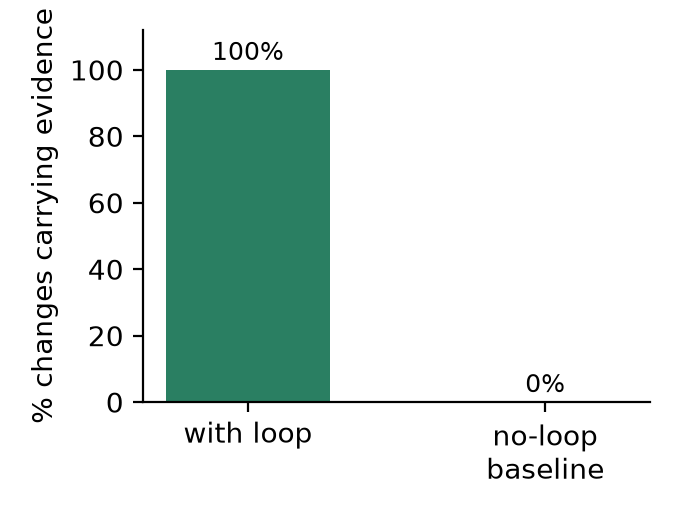
\includegraphics[width=0.47\columnwidth]{figures/evidence_rate.png}%
\hfill
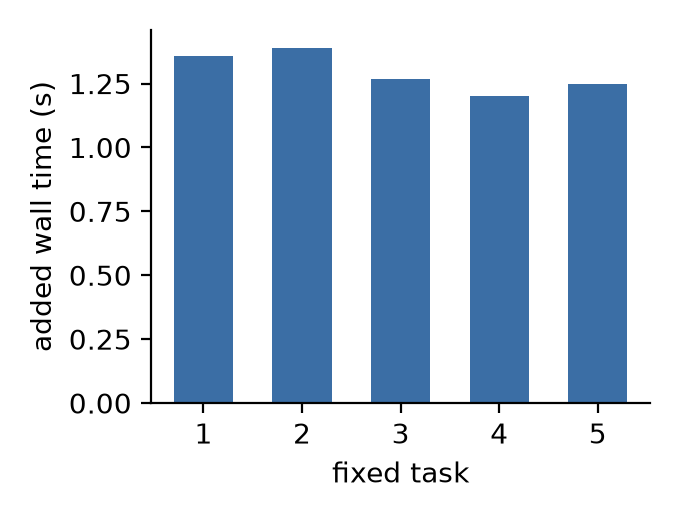
\includegraphics[width=0.47\columnwidth]{figures/overhead.png}
\caption{Left: share of applied managed-file changes carrying evidence,
under the loop versus an ungoverned baseline. Right: added wall time per
change across the fixed tasks. Both figures are regenerated by
\texttt{make reproduce} from the same logs as Table~\ref{tab:metrics}.}
\label{fig:results}
\end{figure}

\subsection{Governance overhead and evidence discipline}
Across \overheadTasks{} fixed managed-file changes, the loop added a mean
of \overheadSeconds~s of wall time per change versus a direct edit; the
loop operations are deterministic code and add zero model tokens, so the
only recurring model-context cost is the skill body plus the
\texttt{AGENTS.md} block ($\approx$\overheadTokens{} tokens). The
discipline it buys is large: under the loop \evLoopRate\% of applied
managed-file changes carried evidence, against \evBaselineRate\% for an
ungoverned baseline session of direct edits (Figure~\ref{fig:results}).
The asymmetry is structural rather than behavioural---the gate refuses an
evidence-free change---which is the point: discipline that depends on
remembering is discipline that erodes.

\subsection{Skill trigger rate}
The consumer door's value depends on the skill firing when a lesson
appears. We measure this with headless prompts against a governed fixture,
counting a run as triggered when the agent proposes through the CLI. This
metric requires a live model and API access and is therefore reported, not
gated: it is excluded from the offline CI gate. Over \triggerN{} headless
sessions the agent routed through the CLI in \triggerRate\% of runs,
against a pre-registered soft floor of \triggerFloor\%. In every run the agent
produced a ChangeSet with evidence rather than editing the managed file
directly. \S\ref{sec:limits} states what this number does and does not
support.

\section{Threats and adversarial results}
\label{sec:threats}
The adversarial suite performs each attack for real against the binary and
passes only if the system stops or detects it. \textbf{T1} pushes
self-graded evidence at L2 (refused by I3). \textbf{T2} uses injected
content to drive a proposal at a non-allowlisted memory
path~\cite{minja} (refused by I4, journaled). \textbf{T4} attempts loop
self-capture---editing the policy (refused by I1) and hand-editing the
journal (caught by \texttt{verify}). \textbf{T5} induces a plausible
capability backdoor: it lands in the L1 queue, never auto-applies, and its
diff and rationale surface for review. \textbf{T6} tampers a journal line
(caught at the exact entry by the hash chain). A Team-lite supply-chain
test tampers a ChangeSet in the registry, refused on pull by signature
verification. All \advDetections{} modelled threats were stopped. Crucially
a \textbf{control}---a legitimate, well-evidenced change---passed the same
gates and applied, so the gates are not theatre that blocks everything.

\section{Limitations}
\label{sec:limits}
This work is deliberately scoped, and honesty about the edges matters more
than breadth.
\begin{itemize}[leftmargin=1.2em,itemsep=1pt]
\item \textbf{Team-lite, not full Team.} Signing is detached
  \texttt{ed25519}, not Sigstore keyless signing with in-toto
  provenance~\cite{sigstore,intoto}. The registry is a git remote, not an
  OCI registry.
\item \textbf{Governed profile is specified, not implemented.} The
  transparency-log journal, policy-as-code gates, and the regulatory export
  mapping to the EU AI Act~\cite{euaiact}, FDA PCCP~\cite{fdapccp},
  ISO/IEC~42001~\cite{iso42001}, and the NIST AI RMF~\cite{nistairmf} are
  described in the spec but not built in v1.
\item \textbf{Single-model, small-$n$ trigger data.} The skill trigger rate
  was measured over \triggerN{} headless sessions with one model family and
  five hand-written lesson prompts. \triggerRate\% is a clean result, but
  $n$ is small, the prompts state the lesson explicitly, and the fixture is
  synthetic---so this measures whether an instructed agent \emph{can} and
  \emph{does} route through the loop, not how often a lesson is
  spontaneously recognised mid-task. It should be read as indicative.
  Reaching this number also required pre-trusting the fixture workspace and
  allowlisting the CLI: without those, headless sessions described the
  correct commands instead of running them, which measures the sandbox
  rather than the skill.
\item \textbf{Scenario fixtures are small.} They are real projects driven
  by the real binary, but they are not large production repositories.
\item \textbf{Weight updates are opaque.} The standard records a weight
  swap; it does not evaluate or gate the weights themselves.
\item \textbf{Actor identity is asserted, not proven.} The Core executor
  enforces that a reviewer is not the producer, but it cannot authenticate
  that a \texttt{human/} actor is a human---the identity is a string the
  caller supplies. We hit this while dogfooding: a rollback in this
  project's own journal is attributed to a human who did not perform it.
  Because the journal is append-only, the mistaken entry remains in the
  record rather than being quietly corrected, which is the intended
  behaviour but also shows the limit. Signed journal entries (Governed
  profile) are the answer, and v0.1 additionally defines no annotation
  event with which a later entry could formally supersede an earlier
  claim.
\end{itemize}

\section{Related work}
\label{sec:related}

\paragraph{Self-improving agent systems.} Recent systems modify their own
prompts, code, or search procedure: the Darwin G\"odel
Machine~\cite{dgm} evolves agent code against benchmarks,
AlphaEvolve~\cite{alphaevolve} evolves programs for scientific and
algorithmic discovery, and GEPA~\cite{gepa} evolves prompts through
reflection. DSPy~\cite{dspy} compiles declarative pipelines into optimized
programs. These systems answer \emph{how to generate} an improvement; none
defines a portable, gated, auditable representation of \emph{one}
improvement, which is the gap this work addresses. The relationship is
complementary: each becomes a Producer through a thin exporter, and their
outputs become comparable and governable without changing how they search.
The DGM result also motivates our sharpest rule: a system that generates
its own improvements must not also be the only judge of them~\cite{dgm}.

\paragraph{Supply-chain integrity.} in-toto~\cite{intoto} and
SLSA~\cite{slsa} define how to attest that an artifact came from a
declared process; Sigstore~\cite{sigstore} makes signing practical at
scale. We borrow their shape---a signed, verifiable claim travelling with
an artifact---and apply it to agent self-modification, where the
``artifact'' is a change to the files that steer an agent. Our Team-lite
profile implements the minimum useful subset; the full profile is
specified in terms of these systems rather than reinventing them.

\paragraph{Transparency logs.} Certificate Transparency~\cite{rfc6962}
established append-only Merkle logs as the way to make a record
tamper-evident rather than merely trusted. The Core journal is the
lightweight analogue: a hash chain any implementation can verify with a
hash function and no infrastructure. The Governed profile upgrades to a
full transparency log with signed entries.

\paragraph{Agent protocols and governance.} MCP~\cite{mcp} standardises
tool access and A2A~\cite{a2a} standardises agent-to-agent messaging; both
are orthogonal to how an agent changes \emph{itself}. On the governance
side, the EU AI Act~\cite{euaiact}, the FDA's predetermined change control
plans~\cite{fdapccp}, ISO/IEC~42001~\cite{iso42001}, and the NIST AI
RMF~\cite{nistairmf} all require, in different words, a declared envelope
of permitted change plus records of what actually changed. The Policy and
Journal objects are deliberately shaped to map onto that requirement, so
that a compliance-facing export is a rendering problem rather than a
redesign.

\paragraph{Attacks on agent memory.} MINJA~\cite{minja} shows that an
attacker can poison an agent's memory through ordinary interaction. This is
precisely the class our context-layer gating targets: memory writes become
proposals that must clear an allowlist and carry evidence, and every
attempt is journaled whether or not it succeeds.

\section{Future work}
\label{sec:future}
Three directions matter most. First, the Governed profile: a
transparency-log journal with signed entries, gates expressed in a policy
language, and an auditor-facing export mapped to the regimes above. Second,
independent implementations: the conformance suite exists so that a second
and third executor, written by other people, can exchange one ChangeSet;
that exchange is the real test of the interoperability claim. Third,
measurement at scale: multi-model trigger studies, larger repositories, and
a proposed OpenTelemetry ``self-modification span'' so that governed change
becomes visible in ordinary telemetry~\cite{otelgenai}.

\section{Conclusion}
An improvement that is proven, gated, recorded, reversible, and portable
can travel: an agent on runtime A learns a lesson, and by the time a second
runtime runs, it carries that lesson---because the lesson moved as a signed
ChangeSet, carried evidence, passed policy, entered the journal, and shipped
through the registry, and an auditor can reconstruct all of it from the
journal alone.

\bibliographystyle{plain}
\begin{thebibliography}{99}
% References. Every entry was verified against a live authoritative source
% on 2026-08-31 (arXiv, DOI, RFC Editor, EUR-Lex, or the official project
% site). See paper/CITATIONS.md for the verification record. No entry is
% marked [VERIFY]: none was unconfirmed.

\bibitem{dgm}
J.~Zhang, S.~Hu, C.~Lu, R.~Lange, and J.~Clune.
\newblock Darwin G\"odel Machine: Open-Ended Evolution of Self-Improving Agents.
\newblock arXiv:2505.22954, 2025. \url{https://arxiv.org/abs/2505.22954}

\bibitem{alphaevolve}
A.~Novikov et~al.
\newblock AlphaEvolve: A Coding Agent for Scientific and Algorithmic Discovery.
\newblock arXiv:2506.13131, 2025. \url{https://arxiv.org/abs/2506.13131}

\bibitem{gepa}
L.~A. Agrawal et~al.
\newblock GEPA: Reflective Prompt Evolution Can Outperform Reinforcement Learning.
\newblock arXiv:2507.19457, 2025. \url{https://arxiv.org/abs/2507.19457}

\bibitem{dspy}
O.~Khattab, A.~Singhvi, P.~Maheshwari, Z.~Zhang, K.~Santhanam, S.~Vardhamanan,
S.~Haq, A.~Sharma, T.~T. Joshi, H.~Moazam, H.~Miller, M.~Zaharia, and C.~Potts.
\newblock DSPy: Compiling Declarative Language Model Calls into Self-Improving Pipelines.
\newblock In \emph{ICLR}, 2024. arXiv:2310.03714.

\bibitem{minja}
S.~Dong, S.~Xu, P.~He, Y.~Li, J.~Tang, T.~Liu, H.~Liu, and Z.~Xiang.
\newblock A Practical Memory Injection Attack against LLM Agents (MINJA).
\newblock arXiv:2503.03704, 2025. \url{https://arxiv.org/abs/2503.03704}

\bibitem{intoto}
S.~Torres-Arias, H.~Afzali, T.~K. Kuppusamy, R.~Curtmola, and J.~Cappos.
\newblock in-toto: Providing Farm-to-Table Guarantees for Bits and Bytes.
\newblock In \emph{USENIX Security}, pages 1393--1410, 2019.

\bibitem{slsa}
Open Source Security Foundation.
\newblock Supply-chain Levels for Software Artifacts (SLSA), Specification v1.2, 2025.
\newblock \url{https://slsa.dev/spec/v1.2/}

\bibitem{sigstore}
Z.~Newman, J.~S. Meyers, and S.~Torres-Arias.
\newblock Sigstore: Software Signing for Everybody.
\newblock In \emph{ACM CCS}, pages 2353--2367, 2022. doi:10.1145/3548606.3560596.

\bibitem{inspect}
UK AI Security Institute.
\newblock Inspect: An Open-Source Framework for Large Language Model Evaluations, 2024.
\newblock \url{https://inspect.aisi.org.uk/}

\bibitem{lmeval}
L.~Gao et~al.
\newblock The Language Model Evaluation Harness (v0.4.3).
\newblock Zenodo, 2024. doi:10.5281/zenodo.12608602.

\bibitem{otelgenai}
OpenTelemetry Authors (CNCF).
\newblock Semantic Conventions for Generative AI Systems, 2025.
\newblock \url{https://opentelemetry.io/docs/specs/semconv/gen-ai/}

\bibitem{agentsmd}
AGENTS.md Contributors.
\newblock AGENTS.md: An Open Format for Guiding Coding Agents, 2025.
\newblock \url{https://agents.md/}

\bibitem{mcp}
Anthropic.
\newblock Model Context Protocol Specification, 2024--2026.
\newblock \url{https://modelcontextprotocol.io/specification}

\bibitem{a2a}
A2A Project (Linux Foundation).
\newblock Agent2Agent (A2A) Protocol Specification, Version 1.0.0, 2026.
\newblock \url{https://a2a-protocol.org/latest/specification/}

\bibitem{rfc2119}
S.~Bradner.
\newblock Key Words for Use in RFCs to Indicate Requirement Levels.
\newblock RFC 2119 (BCP 14), IETF, March 1997. doi:10.17487/RFC2119.

\bibitem{euaiact}
European Parliament and Council of the European Union.
\newblock Regulation (EU) 2024/1689 (Artificial Intelligence Act).
\newblock Official Journal of the European Union, July 2024.
\newblock \url{https://eur-lex.europa.eu/eli/reg/2024/1689/oj/eng}

\bibitem{fdapccp}
U.S. Food and Drug Administration.
\newblock Marketing Submission Recommendations for a Predetermined Change
Control Plan for Artificial Intelligence-Enabled Device Software Functions.
\newblock Final guidance, December 2024.

\bibitem{iso42001}
ISO/IEC.
\newblock ISO/IEC 42001:2023 --- Information Technology --- Artificial
Intelligence --- Management System.
\newblock ISO, 2023.

\bibitem{nistairmf}
National Institute of Standards and Technology.
\newblock Artificial Intelligence Risk Management Framework (AI RMF 1.0).
\newblock NIST AI 100-1, 2023. doi:10.6028/NIST.AI.100-1.

\bibitem{rfc6962}
B.~Laurie, A.~Langley, and E.~Kasper.
\newblock Certificate Transparency.
\newblock RFC 6962, IETF, June 2013. doi:10.17487/RFC6962.
\newblock Obsoleted by RFC 9162 (CT v2.0).

\end{thebibliography}

\end{document}
